\section*{Microwave transitions in laser-cooled alkali metals}

\begin{frame}{Working principle}

    Atoms cooling is a common technique used to \textbf{mitigate the Doppler broadening} of the atomic transitions and \textbf{reduce the collisional shifts}.

    \begin{figure}
        \centering
        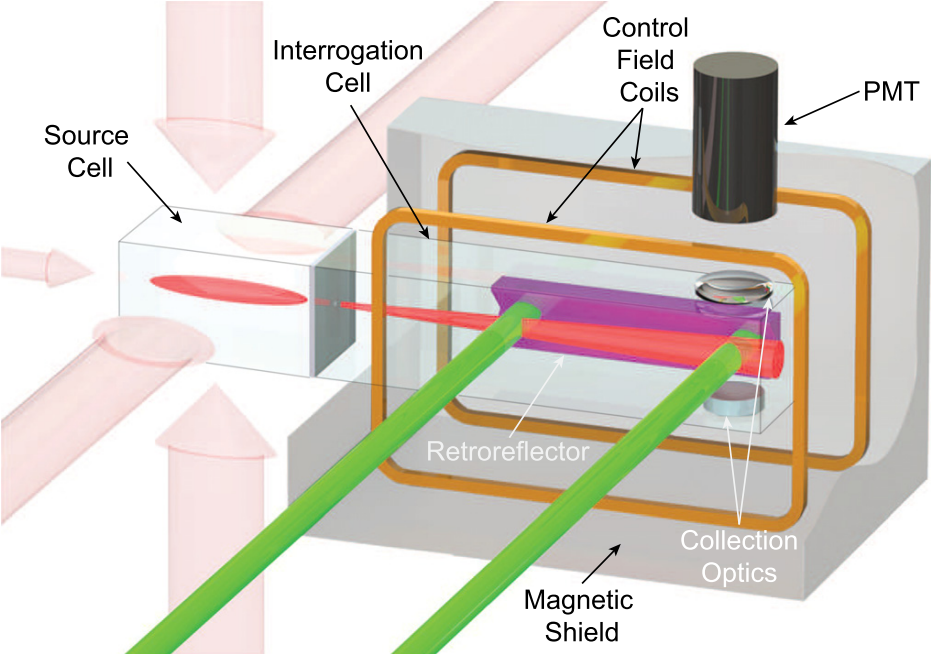
\includegraphics[width=0.6\textwidth]{img/laser-cooled-alkali-metals-trapping.png}
        \caption{Schematic of a 2D-MOT\footnotemark[1] and the interrogation cell.}
    \end{figure}

    \footnotetext[1]{2D-MOT: 2D Magneto-Optical Trap}
    \footnotetext[2]{PMT: Photo-Multiplier Tube}

\end{frame}



\begin{frame}{Current results}

    Stability results look promising but as of today the main bottlenecks are given by the \textbf{technological and experimental limitations}.
    A consistent advancement in those areas is needed to make this technology a viable solution for the future.

    \begin{columns}[T, onlytextwidth]

        \begin{column}{0.5\textwidth}

            \begin{figure}
                \centering
                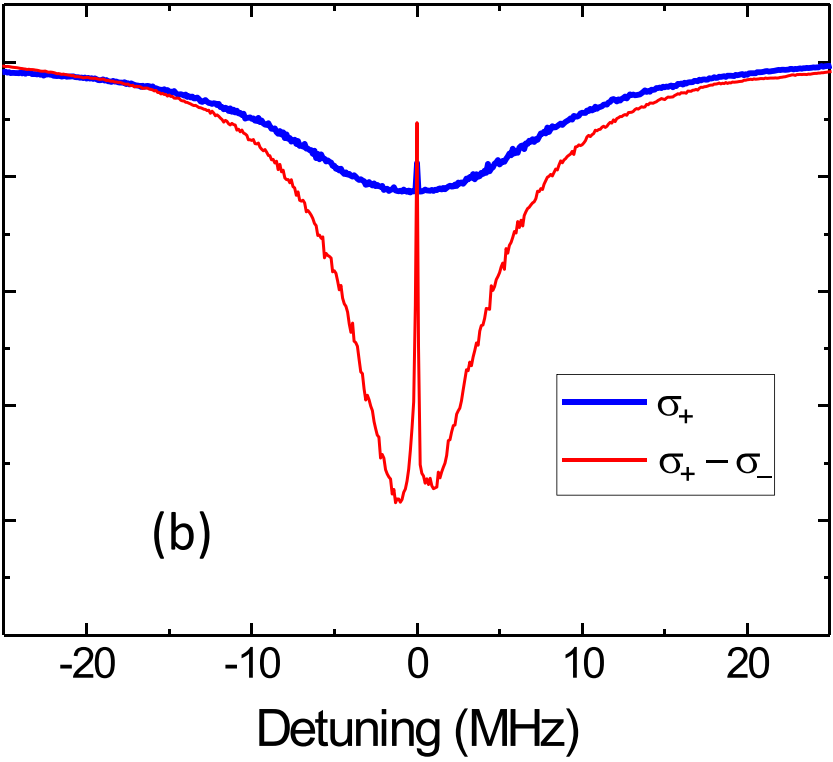
\includegraphics[height=0.45\textheight]{img/laser-cooled-alkali-metals-trasmission.png}
                \caption{\textcolor[HTML]{CA0200}{Laser-cooled} vs. \textcolor[HTML]{3700A7}{traditional} CSAC transmission.}
            \end{figure}

        \end{column}

        \begin{column}{0.5\textwidth}

            \begin{figure}
                \centering
                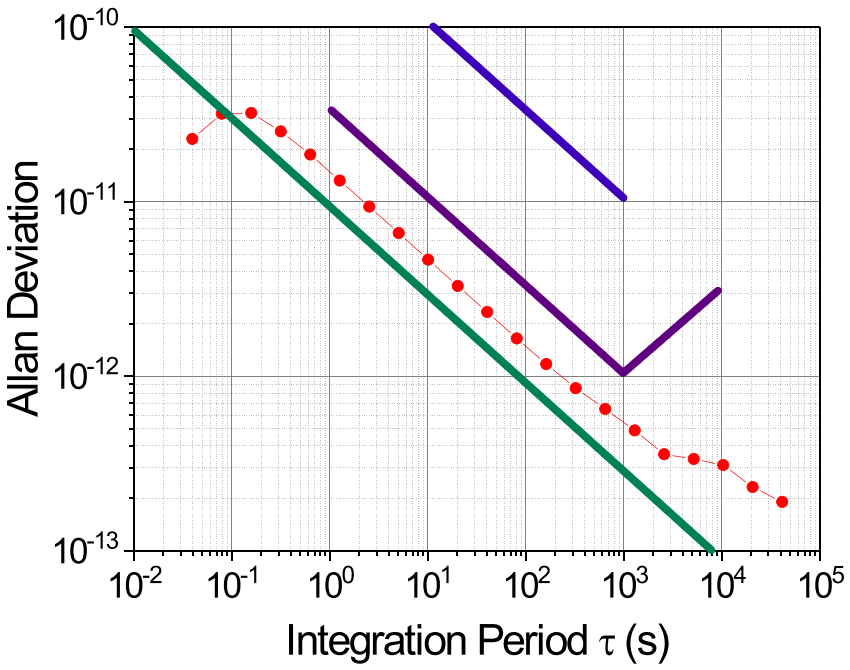
\includegraphics[height=0.45\textheight]{img/laser-cooled-alkali-metals-stability.png}
                \caption{
                    \textcolor[HTML]{006C43}{Target},
                    \textcolor[HTML]{4C0062}{SA.55 MAC},
                    \textcolor[HTML]{3700A7}{SA.45s CSAC},
                    \textcolor[HTML]{CA0200}{Laser-cooled CSAC}
                }
            \end{figure}

        \end{column}

    \end{columns}

\end{frame}